\chapter{Scientific Problem}
\label{section:scientificProblem}

\section{Problem definition}
\label{section:problemDefinition}
The purpose of the research in this thesis consists in approaching some alternative methods to replace classic file scanning techniques. Particularly, our target is to demonstrate that Machine Learning algorithms can be used as an efficient mechanism for malicious PDF files detection. Additionally, we want to present a framework that can remotely analyze suspicious PDF files by applying earlier mentioned performant algorithms. This framework has several advantages: 
\begin{itemize}
    \item Takes on the complicated task of applying classification model for uploaded files and giving the analysis result to the users.
    \item It is designed to be deployed as a Cloud Application on a powerfull server that can handle multiple requests at the same time, lacking users care about having high specifications for their computers.
    \item Guarantees the privacy of the scanned documents. The algorithms doesn't require the documents content in order to decide whether they are malicious or benign. Also, after analysis process, none of the documents are stored on the Cloud.
    \item Keeps the detection algorithms up-to-date. It won't be the users responsability anymore to regularly update the software antivirus installed on their computers. 
    \item Provides a generic implementation for analyzing uploaded files. The support for a new file extension to be scanned, can be effortlessly added by adding a classifier Machine Learning model for the wanted file format.
\end{itemize}
Integrating both Machine Learning and Cloud Computing into Cybersecurity should provide a significant progress to this field. \par


In order to fully automate the process of detection malicious PDF files, our application provides a tool (currently has support only for Microsoft Windows) that independently uploads detected files to the Cloud Service, waits for analysis results and takes appropiate protective measures. In the following we will introduce some operating system concepts that helped us to achieve the expected behavior for our application.

\section{Background processes in Microsoft Windows}
\label{section:backgroundProc}
% https://www.2brightsparks.com/resources/articles/understanding-sessions-in-windows.html
In computing, a background process is a process\footnote{a container for a set of resources used when executing the instance of the program} that runs independently and doesn't require any user involvement. Usually it has the task of system monitoring and sending any types of notifications to the user. Each operating system has its own principle of implementation for background processes. We will have an in-depth look at background processes in Microsoft Windows, which are called \textbf{Windows Services}. According \cite{winInternals} these services are started by a central utility - \textit{Services Control Manager} at the boot-time\footnote{the period when a computer is starting} of the computer and they don't have any graphical interface. For security and safety reasons, specifically to prevent user applications from accessing Windows Services that could run with high privileges, Windows OS creates a new session for each logged in user, reserving \textit{Session 0} for non-interactive services. The mentioned features make Windows Services suitable for long-running functionality, whose operation doesn't interesect with other users work on the same computer. The support for creating a service is provided by \textbf{.NET Framework}, its features being possible to access by using one of Microsoft's high-level programming language \CSharp.

\section{File System monitoring}
\label{section:filesystem}
In the field of operating systems, a file system is aimed to store data in form of files in a long-term storage. Before being stored on physical devices, data that is created and saved by applications in User-Mode, goes through a chain of drivers from Kernel-Mode. This principle is adopted in many operating systems, inclusively in Microsoft Windows (see Figure \ref{filterDriver}). In order to track every change on the computer's file system, we need a monitoring mechanism. Throughout the development of Windows, serveral technologies have been implemented for integration by software engineers, including: File System Filter Drivers, Update Sequence Number Journal (\textit{USN Journal}), Event Tracing for Windows (\textit{ETW}), \textit{FileSystemWatcher} Class from .NET. In this section we are focusing on two of the most popular Windows file system monitoring mechanisms: Minifilter drivers managed by \textit{Filter Manager} and \textit{FileSystemWatcher}. \par
\textbf{Windows Filter Manager} is a Kernel-Mode driver that intercepts every file system I/O operation and can extend the functionality of the requested operation through each minifilter driver that is registered to it (see Figure \ref{filterDriver}). The order of attachement of each minifilter is identified by an altitude\footnote{unique identifier assigned by Microsoft that determines when a minifilter is loaded}, thus avoiding interleaving the functionality of callback routines of each minifilter. Windows Driver Kit (\textit{WDK}) provides the necessary SDK\footnote{collection of software development tools} for developing minifilter drivers, which are most suitable for Backup agents, Encrpytion managers and Antivirus filters. For more details consult \cite{msdn}. \par

\begin{figure}[H]
	\centerline{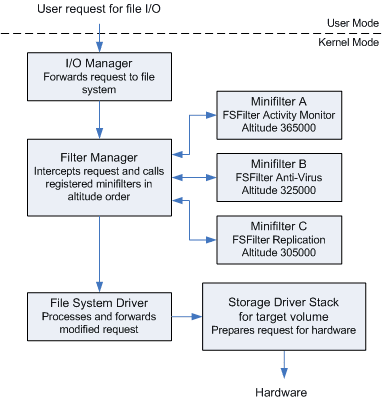
\includegraphics[scale=0.6]{figures/filterDriver.png}}  
	\caption{Simplified I/O stack from Windows \cite{msdn}}
	\label{filterDriver}
\end{figure}

Compared to the previous described technology, which is complex for development and mantaining, \textbf{FileSystemWatcher} is a class from .NET that makes file system monitoring straightforward to implement. According to \cite{dotNetFramework}, this class represents a wrapper over Win32 SDK \textit{ReadDirectoryChangesW} function, which is also used by Windows Explorer to monitor folder changes. By being provided by .NET, it is clear, that FileSystemWatcher can be used in User-Mode for development (see Figure \ref{netFramework}). 

\begin{figure}[H]
	\centerline{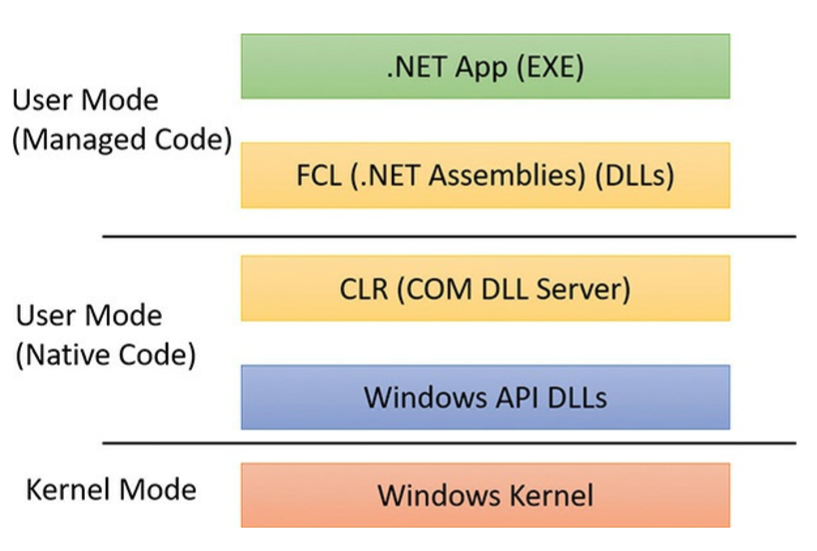
\includegraphics[scale=0.5]{figures/NetFramework.png}}  
	\caption{Relationship between .NET and Windows OS \cite{winInternals}}
	\label{netFramework}
\end{figure}

To configure a working instance of this class, we need to specify a couple of properties, such as \textit{Path} (for indicating the folder to monitor), \textit{NotifyFilters} (for specifieng what kind of file changes to monitor) and \textit{EnableRaisingEvents} (to start/stop monitoring process). Also we need to attach the corresponding events that we want to receive (see Table \ref{table:supportedEvents}).

\begin{table}[H]
	\caption{Events supported by FileSystemWatcher}
	\label{table:supportedEvents}
		\centering
            \begin{tabular}{l | l}
                
				\textbf{Event} & \textbf{Occuring time} \\
				\hline 
 				Created & When a new file is created or is moved into monitored folder \\
 				Changed & When a file has its content or file attributes modified \\
 				Deleted & When a file is removed or is moved out of monitored folder \\
                Renamed & When the name of the file get changed \\
                 
			\end{tabular}
\end{table}

Earlier we mentioned that minifilter drivers live in Kernel-Mode, while FileSystemWatcher provided by .NET lives in User-Mode. One more argument in favor of FileSystemWatcher, besides the high level object-oriented programming language \CSharp that we have at our disposal over unmanaged\footnote{code executed directly by OS; does not provide any security to the application} C language, is that it's safer to run applications in User-Mode. Each application runs in isolation in User-Mode and in case of a crash, it won't affect other applications or even worse the OS itself, what can happen with a Kernel-Mode driver. Even the smallest error that occurs in a driver can cause BSOD\footnote{"Blue Screen of Death", error screen displayed by Windows in case of fatal system crash}. 

\newpage
\section{Analyzing PDF File Structure}
\label{section:pdfStructure}
In this section we are going to understand PDF structure which is a foundation stone of identifieng backdoors\footnote{a malicious method by which a system bypass is hidden} in this file format. \par
PDF was first developed by Adobe in the 1990's with many version been released afterwards. Its initial purpose was to allow to present various types of data, including: text, images, webpage links etc. regardless of the environments it was opened in. As explained in \cite{pdfReference}, PDF files consist of objects, which are of eight types: Boolean values, Numbers (integer and real), Strings, Names, Arrays, Dictionaries, Streams and the Null object. Each PDF document should begin with a header that identifies it as a \textit{PDF} and includes the version number \code{\%PDF-1.7}. The document should also end in a certain way - with the signature \code{\%\%EOF} (see Figure \ref{pdfSkeleton}). After header the objects are declared, that can contain necessary information for rendering the document. One of the most important objects is the stream, that can store an unlimited size sequence of bytes. Usually streams are used for storing text, but they can also store executable code, i.e., checkbox for agreement of \textit{Terms and Conditions}. Streams can contain the optional entry \code{/Filter}, which is aimed for compression and encryption of data inside streams. Next comes the Cross-Reference Table (\textit{Xref}), which 
determines the location of existing objects in PDF. The last section of the file is \textit{Trailer}, that contains the metadata of the file, e.g., size of the file, number of objects, the id of the root object, etc. Hence it becomes clear, that PDF documents are parsed from the end to the start.

\begin{figure}[H]
	\centerline{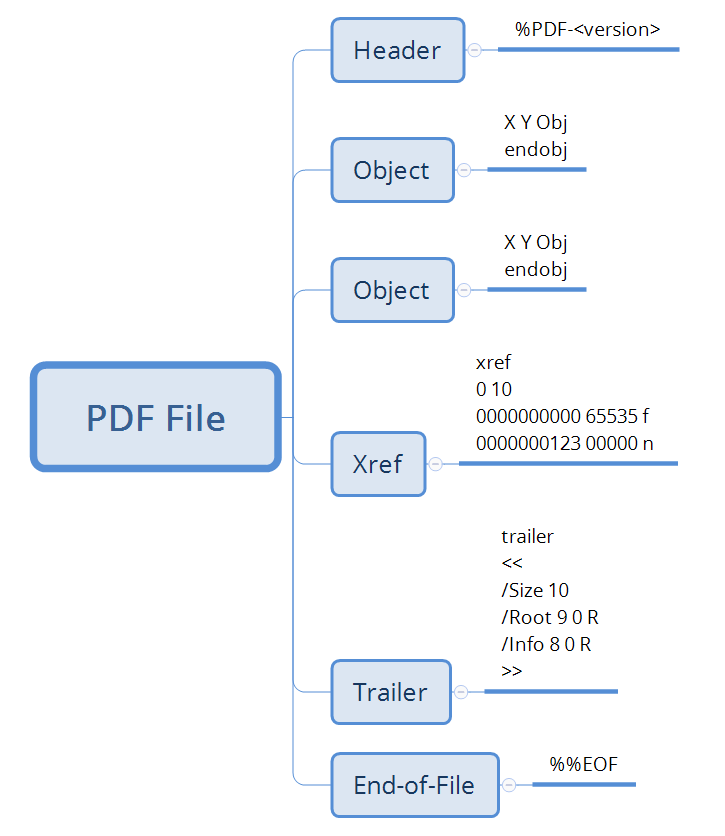
\includegraphics[scale=0.4]{figures/PDFSkeleton.png}}  
	\caption{Structure of PDF Format \cite{logrhythm}}
	\label{pdfSkeleton}
\end{figure}


\section{Malware in PDF}
\label{section:malwareInPDF}
Over the years PDF format has evolved and now it has support not just for text and images, but also for editable forms, animations and even 3D graphics. All of these features made PDF a great solution for information sharing. Meanwhile it also became a good target for cybercriminals, malware being easily embedded into PDF documents and widespread through different types of communication, e.g., HTTP, emails, etc. (see Figure \ref{pdfmalware})

\begin{figure}[H]
	\centerline{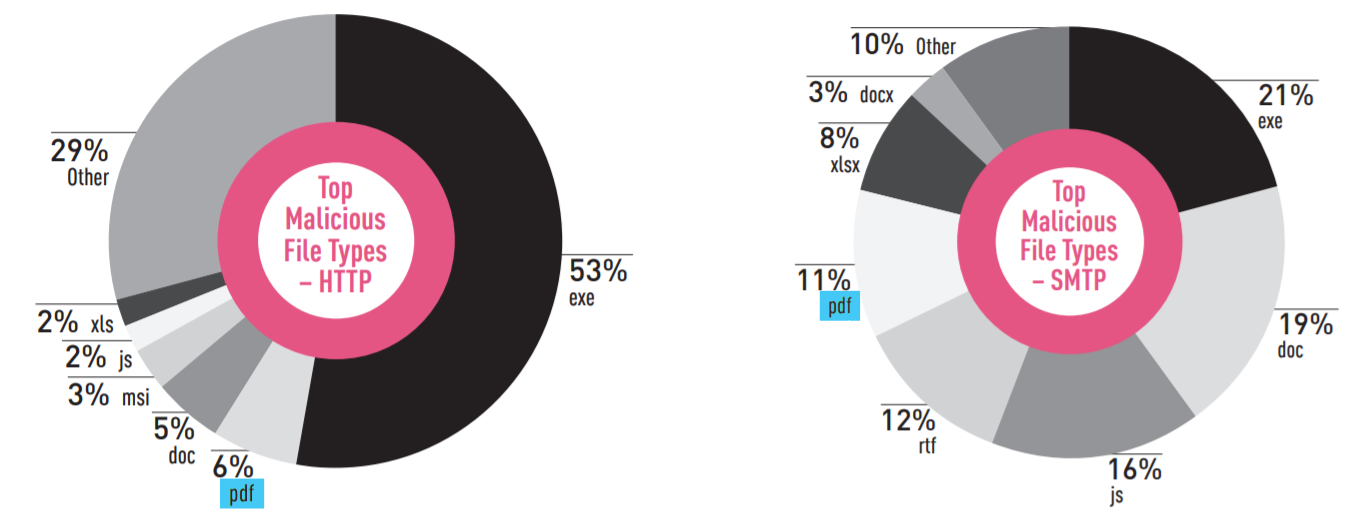
\includegraphics[scale=0.5]{figures/maliciousPDF.png}}  
	\caption{Top malicious file types - H1 2019 \cite{pdfattack}}
	\label{pdfmalware}
\end{figure}

Malicious PDF can be classified into three categories: \textit{reader exploitation}, \textit{feature abuse}, \textit{phishing attacks}. Every year numerous vulnerabilities related to most used PDF readers, e.g., Adobe Reader, Acrobat Reader, Chrome, are reported. Before these weaknesses are patched\footnote{applying changes to fix bugs or errors in a software program}, attackers create exploits to execute arbitrary code, when PDF is opened with one of the vulnerable application. Phishing attacks are more difficult to detect, because in the context of PDF documents, they aren't infected, instead the social engineering is used in order to psychologically enforce someone to click on malicious links written in the documents. Another frequently used attack vector involves misusing the PDF extra-functionalities, such as running malicious code when file is opened, stealing sensitive information and sending to remote addresses, downloading infected executables and so on. Pursuant to \cite{xakepPDF}, it's usually the fault of embedded Javascript code, whose intentions could be wrong, but as seen in Table \ref{table:pdfentries} there are also several standard PDF entries, which seem to be interesting in terms of malware hunting. However, when searching for them we should not forget about the possibility of obfuscation using hex code, in which, for example, \code{/Launch} can turn into \code{/L0x61unc0x68}. Encrypting the streams and strings is another often applied "trick" to complicate the analysis work for both antiviruses and researchers. A PDF document from which it is impossible to copy text or which can not be printed, is such a obfuscated sample.

\begin{table}[H]
	\caption{Standard PDF Entries whose functionality can be abused}
	\label{table:pdfentries}
		\centering
            \begin{tabular}{p{7cm} | p{8cm}}
                
				\textbf{Entry} & \textbf{Functionality} \\
				\hline 
				\code{/JavaScript} & Sets JavaScript code to be executed \\
 				\code{/OpenAction}, \code{/Names}, \code{/AcroForm}, \code{/Action}, \code{/AA} & Defines a script or an action to be automatically run \\
 				\code{/Launch} & Runs a program or opens a document \\
 				\code{/URI} & Accesses a resource by its URL \\
 				\code{/SubmitForm}, \code{/GoToR} & Can send data to indicated URL \\
 				\code{/ObjStm} & Hides objects inside Streams \\
                 
			\end{tabular}
\end{table}


\section{Machine Learning for Malware Detection}
\label{section:mlForMalware}
Machine Learning (\textit{ML}) algorithms are increasingly used in various fields of science due to their fast adaptability to the new arising problems. Cybersecurity is one of these areas, where the complexion and the assortment of attacks are daily raising. It becomes convenient to put ML into practice because of the large amount of collected data (application logs, network traffic scans, etc.), which can be processed using statistics techniques and can be transformed into models for making future predictions based on the new incoming inputs. This solution reduces the costs for continuous analysis, leaving the hard work on powerful computers, whose high performance don't require nowadays huge investments. Also it helps businesses more efficient prevent potential threats and automates routine tasks, allowing security teams to focus on implementing new detection techniques to advance ML algorithms. \par 
As presented in \cite{mlsec}, Machine Learning's use cases in security can be splitted into two types: \textit{anomaly detection} and \textit{pattern recognition}, thus these solutions are used to solve following specific security issues: spam detection (filters are applied on emails, webpages in order to detect patterns of usual phishing attacks), malware catching (polymorphic malwares such as Trojan\footnote{malware that is disguised as benign software to avoid detection}, Spyware\footnote{malware that is aimed to collect information without permission of the user}, Ransomware\footnote{malware that restricts access to personal data} etc. is recognized based on their behavior), account takeover spot (such kind of anomaly is detected, because of multiple tries when gaining access to someone's account) and many others. For more detailed information about used Machine Learning techniques in Cybersecurity consult Table \ref{table:mlAlgos}.

\begin{table}[H]
	\caption{Application of Machine Learning to Cybersecurity problems}
	\label{table:mlAlgos}
		\centering
            \begin{tabular}{p{3cm} || p{5cm} | p{3cm} | p{4cm}}
                
				\textbf{Technique} & \textbf{Explanation} & \textbf{Algorithm} & \textbf{Cybersecurity problem} \\
				\hline \hline
				\texttt{Classification} & Separation into different categories & K-Nearest Neighbors (\code{KNN}), Support Vector Machine(\code{SVM}), Random Forest & Spam filtering \\
				\hline
				\texttt{Regression} & Prediction of future values based on previous ones & Linear Regression (\code{LR}) & Fraud detection \\
				\hline
				\texttt{Association Rule Learning} & Recommendation based on past experience & Equivalence Class Clustering and bottom-up Lattice Traversal (\code{ECLAT}) & Incident response (suggest a policy to apply in case of a particular incident) \\
				\hline
				\texttt{Clustering} & Grouping into unknown categories based on similar features & \code{K-Means} & Detection of polymorphic malwares \\
				\hline
				\texttt{Generative Model} & Generation based on known distribution & Markov Chains & Vulnerability scanning \\
				
			\end{tabular}
\end{table}

%Over-reliance on AI in cybersecurity can create a false sense of safety, Marty adds. That's why, in addition to judiciously applied algorithms, his firm employs cybersecurity experts, data scientists and psychologists. As with all current artificial intelligence, machine learning supplements and enhances human efforts, rather than replacing them. 

% “AI is going to become more prevalent in security. It's maturing,” CrowdStrike Founder and CEO George Kurtz said in late 2018. “AI is a feature, not a company. It's going to play a role in solving a specific problem. But not every problem can be solved with AI.


% \section{Benefits of Cloud Computing}
% \label{section:cloudComputing}
% Using a cloud-based anti-virus makes it much easier to manage, especially as there's no need to constantly update software on multiple devices. However, it is worth bearing in mind that installing anti-virus to combat malware can only be one part of an overall IT security policy.
% https://www.redhat.com/en/topics/cloud-native-apps/what-are-cloud-applications
% Simply put, a cloud application is software that users access primarily through the internet, meaning at least some of it is managed by a server, not the user’s local machine. This basic definition doesn’t fully describe how cloud applications have reshaped markets and business models, though. If designed well, cloud applications can offer a user experience like a program installed entirely on a local machine, but with reduced resource needs, more convenient updating, and the ability to access functionality across different devices.
% Nowadays with cloud use being common, it's more efficient to install anti-virus software on your network.
% benfetis - low performant devices + mobile
% http://lxiao.xmu.edu.cn/Papers/Mobile%20Offloading%20for%20Cloud-based%20Malware%20Detections%20with%20Learning.pdf
%Advantages:
% Fast computation to run more advanced and complex detection algorithms
% More accurate detection with a large-size signature database
% Address zero-day vulnerabilities
% Cloud-based malware detection vs. local detection
%  Transmission delay, computation speed, detection accuracy, storage cost
%  User competition vs. cooperation in the malware detection
%  Compete for the limited network bandwidth
%  Contribute the malware signature database to improve the malware
%  detection accuracy at the cloud
%Cloud computation resource=1Gbps
% Trace generation speed=1Mbps
% Transmission cost factor=0.2
% Accuracy coefficient=0.5 